\documentclass[logo,reportComp]{thesis}
\usepackage[cpp,pseudo]{mypackage}

\title{计算机图形学}
\subtitle{作业三:星球旋转}
\school{数据科学与计算机学院}
\author{陈鸿峥}
\classname{17大数据与人工智能}
\stunum{17341015}
\headercontext{计算机图形学作业}
% \lstset{language=python}

\begin{document}

\maketitle

本次实验我实现了两个版本的程序,第一个版本采用OpenGL的固定管线进行编写,第二个版本采用可编程着色器的方式进行编写。

\section{固定管线}
双击打开\verb'planet.exe'即可运行,\verb'glut32.dll'为运行所需的库过程。
四种基本操作如下:
\begin{itemize}
	\item 按d键:小星球正方向自转
	\item 按SHIFT+d键:小星球反方向自转
	\item 按y键:小星球绕大星球正方向公转
	\item 按SHIFT+y键:小星球绕大星球反方向公转
\end{itemize}

设小星球与大星球的距离为$d$,则公转$\theta$弧度后小星球的位置为
\[(x,z)=(d\sin\theta, d\cos\theta)\]
在实际做变换时应注意先进行旋转操作,再进行平移,旋转是绕$y$轴旋转。

同时为更好展示$z$轴上的距离远近,我采用了一线性函数,对小星球的半径进行调整。
当小星球离我们更近时,即在$z$轴正向,则半径最大;反之,离我们越远,其显示半径越小。

实验结果如下图所示。
\begin{figure}[H]
\centering
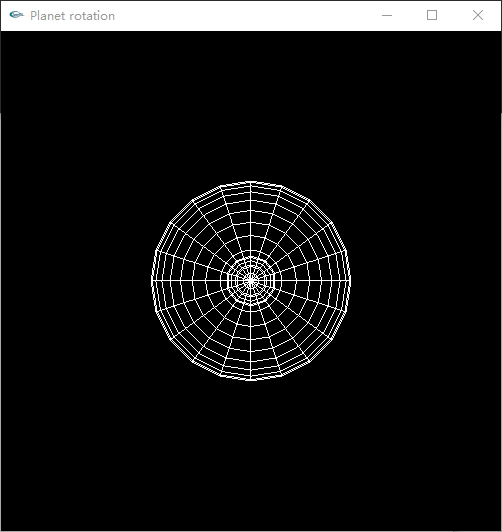
\includegraphics[width=0.6\linewidth]{fig/initial_state.png}
\caption{初始状态}
\end{figure}
\begin{figure}[H]
\centering
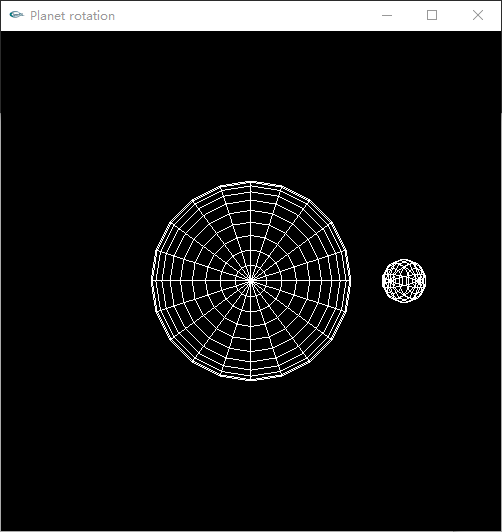
\includegraphics[width=0.6\linewidth]{fig/rotate_state.png}
\caption{旋转后状态}
\end{figure}

实验的代码如下。
\begin{lstlisting}
#include <windows.h>
#include <GL/glut.h>
#include <stdio.h>
#include <math.h>

const double PI = 2*acos(0.0);

int angRot = 0;
int angRevo = 0;
float distance = 0.8;

void myDisplay()
{
    glClear(GL_COLOR_BUFFER_BIT);

    // Big sphere
    glutWireSphere(0.4f, 20, 20);

    float posx = (float) sin((float)angRevo/180*PI) * distance;
    float posz = (float) cos((float)angRevo/180*PI) * distance;

    glPushMatrix(); // only transform smaller one
    // planet revolution
    glTranslatef(posx,0,posz);
    // planet rotation (firstly self rotate)
    glRotatef(angRot,0,1,0);
    // for visualization, the size of the sphere is changed linearly
    glutWireSphere(0.1f*(posz+2*distance)/(3*distance), 8, 8);
    glPopMatrix();

    glFlush();
}

void keyPressed(unsigned char key, int x, int y)
{
    // int mod = glutGetModifiers(); // GLUT_ACTIVE_SHIFT
    printf("Pressed %c!\n", key);
    switch (key){
        case 'd':angRot = (angRot + 10) % 360;break;
        case 'D':angRot = (angRot - 10) % 360;break;
        case 'y':angRevo = (angRevo + 10) % 360;break;
        case 'Y':angRevo = (angRevo - 10) % 360;break;
    }
    myDisplay();
}


int main(int argc, char *argv[])
{
    glutInit(&argc, argv);

    glutInitDisplayMode(GLUT_RGB | GLUT_SINGLE);

    glutInitWindowPosition(100, 100);
    glutInitWindowSize(500, 500);

    glutCreateWindow("Planet rotation");

    glutDisplayFunc(myDisplay);
    glutKeyboardFunc(keyPressed);

    // get into display
    glutMainLoop();

    return 0;
}
\end{lstlisting}
编译指令如下:
\begin{flushleft}
\verb'gcc planet.c -I.\include -L.\lib -lglut32 -lopengl32 -o planet.exe'
\end{flushleft}

\section{着色器编程}
采用着色器的方法进行编程耗费了我大量精力,单单是配置环境就配置了两天,当然最终成功配置并将实验完成还是挺开心的。

双击打开\verb'shader.exe'即可运行,\verb'glut32.dll'和\verb'glew32.dll'为运行所需的库过程。
四种基本操作如下:
\begin{itemize}
    \item 按d键:小星球正方向自转
    \item 按SHIFT+d键:小星球反方向自转
    \item 按y键:小星球绕大星球正方向公转
    \item 按SHIFT+y键:小星球绕大星球反方向公转
\end{itemize}

这里我主要采用顶点着色器对球上的坐标变换进行控制,这里注意变换的粒度是球上的每一个顶点。
注意到无论是自转还是公转都可以看作是绕某一$y$轴旋转的结果,即只需进行如下的2维旋转变换即可
\[\bmat{x'\\y'}=\bmat{\cos\theta & -\sin\theta\\\sin\theta & \cos\theta}\bmat{x\\y}\]
其中$\theta$为旋转的角度,本实验中自转公转都为$10\degree$。

而自转与公转的唯一区别在于需要先进行参考系的变换,使得坐标原点落在小球球心,再套用上述公式,即可完成自转的操作。

相比起固定管线,着色器的程序要麻烦很多,主要经过以下几个步骤:
\begin{itemize}
    \item 创建着色器\verb'glCreateShader'
    \item 添加着色器源代码\verb'glShaderSource'
    \item 编译着色器代码\verb'glCompileShader'
    \item 创建着色器程序\verb'glCreateProgram'
    \item 将顶点与片源着色器依附在上述程序上\verb'glAttachShader'
    \item 链接着色器程序\verb'glLinkProgram'
\end{itemize}
在源程序与着色器之间传递参数采用\verb'glUniform',其他的窗口显示部分则与固定管线类似。

最终实验结果如下图所示,这里为了与上一种方法进行区别,采用了片源着色器将小行星着为黄色。
\begin{figure}[H]
\centering
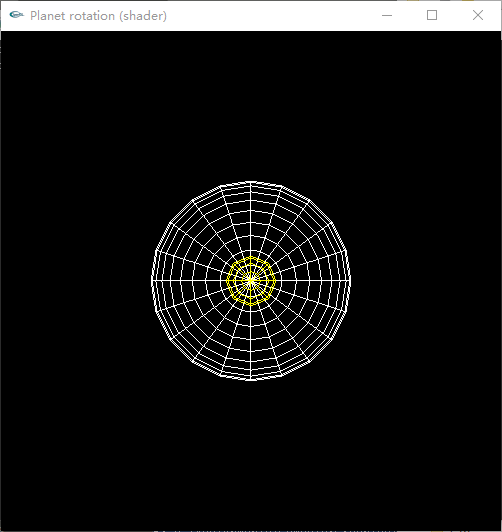
\includegraphics[width=0.6\linewidth]{fig/initial_state_shader.png}
\caption{初始状态(着色器编程)}
\end{figure}
\begin{figure}[H]
\centering
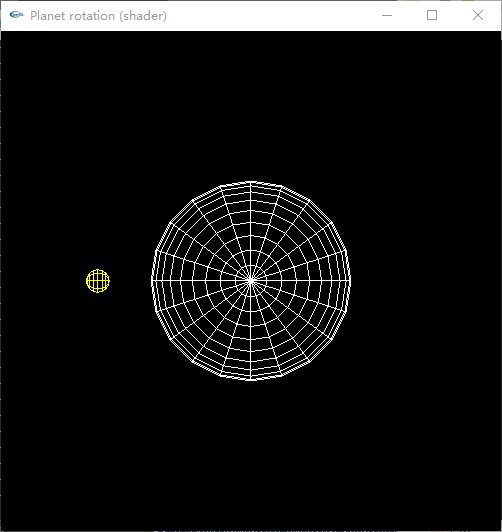
\includegraphics[width=0.6\linewidth]{fig/rotate_state_shader.png}
\caption{旋转后状态(着色器编程)}
\end{figure}

实验的代码如下。
\begin{lstlisting}
#include <windows.h>
#include <stdio.h>
#include <math.h>
#include <GL/glew.h>
#include <GL/glut.h>

const double PI = 2 * acos(0.0);

GLuint smallSphereProgram;
GLuint bigSphereProgram;

int angRot = 0;
int angRev = 0;
float distance = 0.8;

// CIS: \cos(\theta) + i \sin(\theta)
const char* smallVertCode = "layout (location = 0) in vec3 aPos;\n"
"uniform vec2 latCIS;\n"
"uniform vec2 revCIS;\n"
"uniform vec3 center;\n"
"varying vec3 newPos;\n"
"void main()\n"
"{\n"
"  newPos.x = aPos.x * latCIS.y - aPos.z * latCIS.x;\n"
"  newPos.z = aPos.z * latCIS.y + aPos.x * latCIS.x;\n"
"  newPos.x += center.x;\n"
"  newPos.z += center.z;\n"
"  newPos.x = (newPos.x - center.x) * revCIS.y - (newPos.z - center.z) * revCIS.x + center.x;\n"
"  newPos.z = (newPos.z - center.z) * revCIS.y + (newPos.x - center.x) * revCIS.x + center.z;\n"
"  gl_Position = vec4(newPos.x, aPos.y, newPos.z, 1.0f);\n"
"}\n";

const char* smallFragCode = "uniform vec4 newColor;\n"
"void main(void)\n"
"{ gl_FragColor = newColor; }";

const char* bigVertCode = "void main()\n"
"{ gl_Position = ftransform(); }";

const char* bigFragCode = "void main(void)\n"
"{ gl_FragColor = vec4(1,1,1,1); }";

int flag = 0;

void myDisplay()
{
    glClear(GL_COLOR_BUFFER_BIT);

    // Big sphere
    glUseProgram(bigSphereProgram);
    glutWireSphere(0.4f, 20, 20);

    // Small sphere
    glUseProgram(smallSphereProgram); // overwrite
    int vertexColorLocation = glGetUniformLocation(smallSphereProgram,"newColor");
    glUniform4f(vertexColorLocation,1.0f,1.0f,0.0f,1.0f);
    int vertexLatCISLocation = glGetUniformLocation(smallSphereProgram,"latCIS");
    glUniform2f(vertexLatCISLocation,sin((float)angRot/180*PI),cos((float)angRot/180*PI));
    int vertexRevCISLocation = glGetUniformLocation(smallSphereProgram,"revCIS");
    glUniform2f(vertexRevCISLocation,sin((float)angRev/180*PI),cos((float)angRev/180*PI));
    int vertexCenterLocation = glGetUniformLocation(smallSphereProgram,"center");
    float centerx = sin((float)angRev/180*PI) * distance;
    float centerz = cos((float)angRev/180*PI) * distance;
    glUniform3f(vertexCenterLocation,centerx,0,centerz);
    // printf("angRev: %d angRot: %d centerx: %f, centerz: %f\n", angRev, angRot, centerx, centerz);
    glutWireSphere(0.1f*(centerz+2*distance)/(3*distance),8,8);

    glFlush();
}

void keyPressed(unsigned char key, int x, int y)
{
    // int mod = glutGetModifiers(); // GLUT_ACTIVE_SHIFT
    printf("Pressed %c!\n", key);
    switch (key){
        case 'd':angRot = (angRot + 10) % 360;break;
        case 'D':angRot = (angRot - 10) % 360;break;
        case 'y':angRev = (angRev + 10) % 360;break;
        case 'Y':angRev = (angRev - 10) % 360;break;
    }
    myDisplay();
}


int main(int argc, char *argv[])
{
    glutInit(&argc, argv);

    glutInitDisplayMode(GLUT_RGB | GLUT_SINGLE);

    glutInitWindowPosition(100, 100);
    glutInitWindowSize(500, 500);

    glutCreateWindow("Planet rotation (shader)");

    glutDisplayFunc(myDisplay);
    glutKeyboardFunc(keyPressed);

    glewInit();

    int success;
    char infoLog[512];

    // make shader for the small sphere
    GLuint smallVertexShader = glCreateShader(GL_VERTEX_SHADER);
    glShaderSource(smallVertexShader, 1, &smallVertCode, NULL);
    glCompileShader(smallVertexShader);

    glGetShaderiv(smallVertexShader,GL_COMPILE_STATUS, &success);
    if (!success){
        glGetShaderInfoLog(smallVertexShader,512,NULL,infoLog);
        printf("Error: %s\n", infoLog);
    } else
        printf("Successfully compiled!\n");
    GLuint smallFragmentShader = glCreateShader(GL_FRAGMENT_SHADER);
    glShaderSource(smallFragmentShader, 1, &smallFragCode, NULL);
    glCompileShader(smallFragmentShader);

    smallSphereProgram = glCreateProgram();
    glAttachShader(smallSphereProgram,smallVertexShader);
    glAttachShader(smallSphereProgram,smallFragmentShader);

    glLinkProgram(smallSphereProgram);

    // make shader for the big sphere
    GLuint bigVertexShader = glCreateShader(GL_VERTEX_SHADER);
    glShaderSource(bigVertexShader, 1, &bigVertCode, NULL);
    glCompileShader(bigVertexShader);
    glGetShaderiv(bigVertexShader,GL_COMPILE_STATUS, &success);
    if (!success){
        glGetShaderInfoLog(bigVertexShader,512,NULL,infoLog);
        printf("Error: %s\n", infoLog);
    } else
        printf("Successfully compiled!\n");
    GLuint bigFragmentShader = glCreateShader(GL_FRAGMENT_SHADER);
    glShaderSource(bigFragmentShader, 1, &bigFragCode, NULL);
    glCompileShader(bigFragmentShader);

    bigSphereProgram = glCreateProgram();
    glAttachShader(bigSphereProgram,bigVertexShader);
    glAttachShader(bigSphereProgram,bigFragmentShader);

    glLinkProgram(bigSphereProgram);

    // get into display
    glutMainLoop();

    return 0;
}
\end{lstlisting}
编译指令如下:
\begin{flushleft}
\verb'gcc shader.c -I.\include -L.\lib -lopengl32 -lglew32 -lglut32 -o shader.exe'
\end{flushleft}

\end{document}

% 1. 使用 OpenGL 实现简易的星球旋转效果,如图 1。程序执行效果见附带压缩包的 EXE 程序(EXE 文件为 Win 程序,使用Mac OS 和 Linux 的同学请参照Win 平台下的执行效果)。
% 功能要求:
% 1. 使用不同尺寸的线框球体(Wire Sphere)表示大小两个星球;
% 2. 使用平移和旋转操作实现小星球自转和绕大星球旋转的功能,键盘事件响应如下: d 和 shift+d: 分别控制小星球正反两个方向的自转; y 和 shift+y: 分别控制小星球绕大星球的正方向和反方向旋转;
% 3. 语言不限,开发平台不限。具体效果展示允许略有差异。
% 4. 要求使用OpenGL 着色器编程方式实现程序。

% 实现提示: 1. 正方向旋转可以通过以下方式求得:d = (d + 10) % 360;反方向则为 d = (d - 10) % 360
% 要求: 1. 作业按百分制评分,没交作业算 0 分;
% 2. 提交代码文件,缺源代码文件的作业成绩减 10 分;
% 3. 提交直接可执行的程序文件或脚本文件,不能运行的程序(含出错,缺 dll 文件等)作业成绩减 10 分;
% 4. 作业文档,包含简要的程序文件说明,运行方法,以及程序运行结果截图,缺文档的作业成绩减 10 分; 5. 发现作业抄袭的本次作业算 0 分。
% 说明: 以小组为单位,组长收齐小组内各位同学的作业,作业用 zip 格式文件打包提交(请尽量减少压缩包文件的体积),以附件方式发送到课程邮箱:cgcourse_homework@qq.com ,若 2 天内没收到回复,请重新发 邮件。
% 请于 10 月 12 日 24:00 前提交。
% 邮件名和压缩包文件名格式如下: 班级 + 学号 + 姓名 + HW3 例:17 计科+16000001+张三+HW3